% !TeX spellcheck = sk_SK
\chapter{Prehľad existujúcich	metód riadenia pre	Dvojkolesové balansujúce roboty}


Balansujúci robot predstavuje z mechanického hľadiska inherentne nestabilnú sústavu, ktorú je pre to, aby bol takýto robot v praxi použiteľný, potrebné stabilizovať pomocou regulátora. V už existujúcich prácach sa stretávame s rôznymi druhmi implementovaných regulátorov a je teda namieste uviesť aspoň niektoré z najčastejšie používaných. V nasledujúcej časti práce sa teda budeme zaoberať  stručným popisom v praxi používaných regulátorov a uvedieme ako sme sa rozhodovali pri výbere regulátora my.

Vo všeobecnosti môžeme ako regulátor označiť každé zariadenie, ktoré v systéme zabezpečuje udržiavanie určitých fyzikálnych veličín na stanovených úrovniach. V priebehu regulácie sa pravidelne zisťuje skutočný stav objektu a porovnáva sa s požadovaným.  Regulátor následne upravuje stav systému tak, aby bol dosiahnutý požadovaný cieľ.

Jedným zo základných spôsobov rozdelenie regulátorov je na lineárne a nelineárne regulátory. Lineárne regulátory sú určené na riadenie sústav, ktorých prenosové funkcie sa vyznačujú tým, že pre ne platí princíp homogenity a superpozície. Pokiaľ chceme použiť takýto regulátor na riadenie nelineárnej sústavy, t.j. sústavy, pre ktorú neplatí princíp homogenity alebo superpozície, bude takýto regulátor pracovať korektne len ak sústava zotrvá v okolí bodu, kde je možné nájsť jej lineárnu aproximáciu. Tento proces sa nazýva linearizácia. 

Pri nelineárnych regulátoroch táto potreba linearizácie odpadá, keďže regulátory tohto typu dokážu pracovať aj s nelineárnymi sústavami. Nevýhodou práce s nelineárnymi sústavami je ale vyššia náročnosť riešenia nelineárnych diferenčných rovníc. Práve kvôli  tomuto problému existuje v praxi tendencia radšej hľadať spôsoby ako čo najpresnejšie reprezentovať nelineárne systémy lineárnymi diferenčnými rovnicami a následne použiť na ich riadenie lineárny regulátor. Je ale nutné ešte podotknúť, že reálne sa pri zohľadnení všetkých vonkajších vplyvov každá sústava javí ako nelineárna. 

Štúdiom prác, ktoré už boli napísané na tému riadenia dvojkolesového balansujúceho robota sme zistili, že medzi regulátory, ktoré sú najčastejšie pre túto úlohu používané patria lineárne regulátory:
\begin{enumerate}
\item PID (Proportional Integral Derivative Regulator:PID)
\item LQR  (Linear Quadratic Regulator;LQR)
\end{enumerate}

Práve týmito regulátormi sa teda budeme zaoberať v ďalšej podkapitole, no pre úplnosť ešte uvedieme, že vrámci nelineárnych regulátorov sa ako vhodné javia najmä Fuzzy PID a umelé neurónové siete.

\section{Lineárne regulátory}


V tejto časti práce zhrnieme základné poznatky o niektorých vybraných typoch lineárnych regulátoroch. Uvedieme výhodné a nevýhodné vlastnosti jednotlivých regulátorov a v závere zhodnotíme, ktorý sa pre naše potreby javí ako najvhodnejší.

\subsection{PID}


PID regulátor je v praxi najčastejšie používaný regulátor, pričom uplatnenie nachádza  pri riadení veličín ako sú napríklad: teplota, tlak, prietok, poloha, atď. Medzi jeho výhodné vlastnosti patrí najmä robustnosť, jednoduchosť implementácie a možnosť manuálneho naladenia bez potreby použitia zložitých výpočtových techník.  Schematické znázornenie jeho zapojenia v ovládanej sústave je na \figurename~\ref{fig:PIDSchematic}

\begin{figure}
\centering
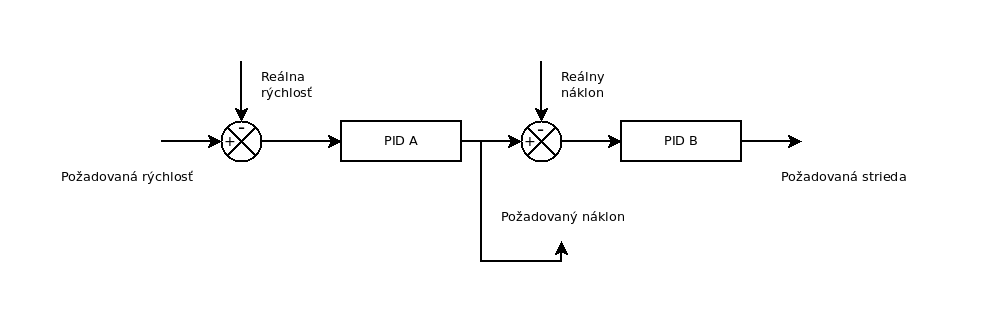
\includegraphics[width=8cm]{PIDSchematic}
\caption{Zapojenie PID}
\label{fig:PIDSchematic}
\end{figure}

Zo schémy je zrejmé, že na vstup privádzame požiadavku na výstup sústavy a od tej následne odčítavame reálne nameranú hodnotu na výstupe (spätná väzba). Takto získavame chybovú veličinu e(t), ktorá vyjadruje nakoľko sa reálna hodnota na výstupe líši od tej požadovanej. Práve s touto chybou ďalej pracuje PID regulátor.

Samotný PID regulátor pozostáva z troch častí, ktoré mu zároveň dávajú jeho názov: proporčnej (P), integračnej (I) a derivačnej (D). Každá s týchto častí iným spôsobom reaguje na vstup do PID a proces ladenia tak pozostáva z nastavenia príslušných parametrov (opísaných nižšie) pre jednotlivé tieto časti. Kombináciou rôznych hodnôt parametrov je možné regulátor naladiť tak, aby podľa potrieb používateľa kontroloval výstupnú veličinu. 

\begin{figure}
\centering
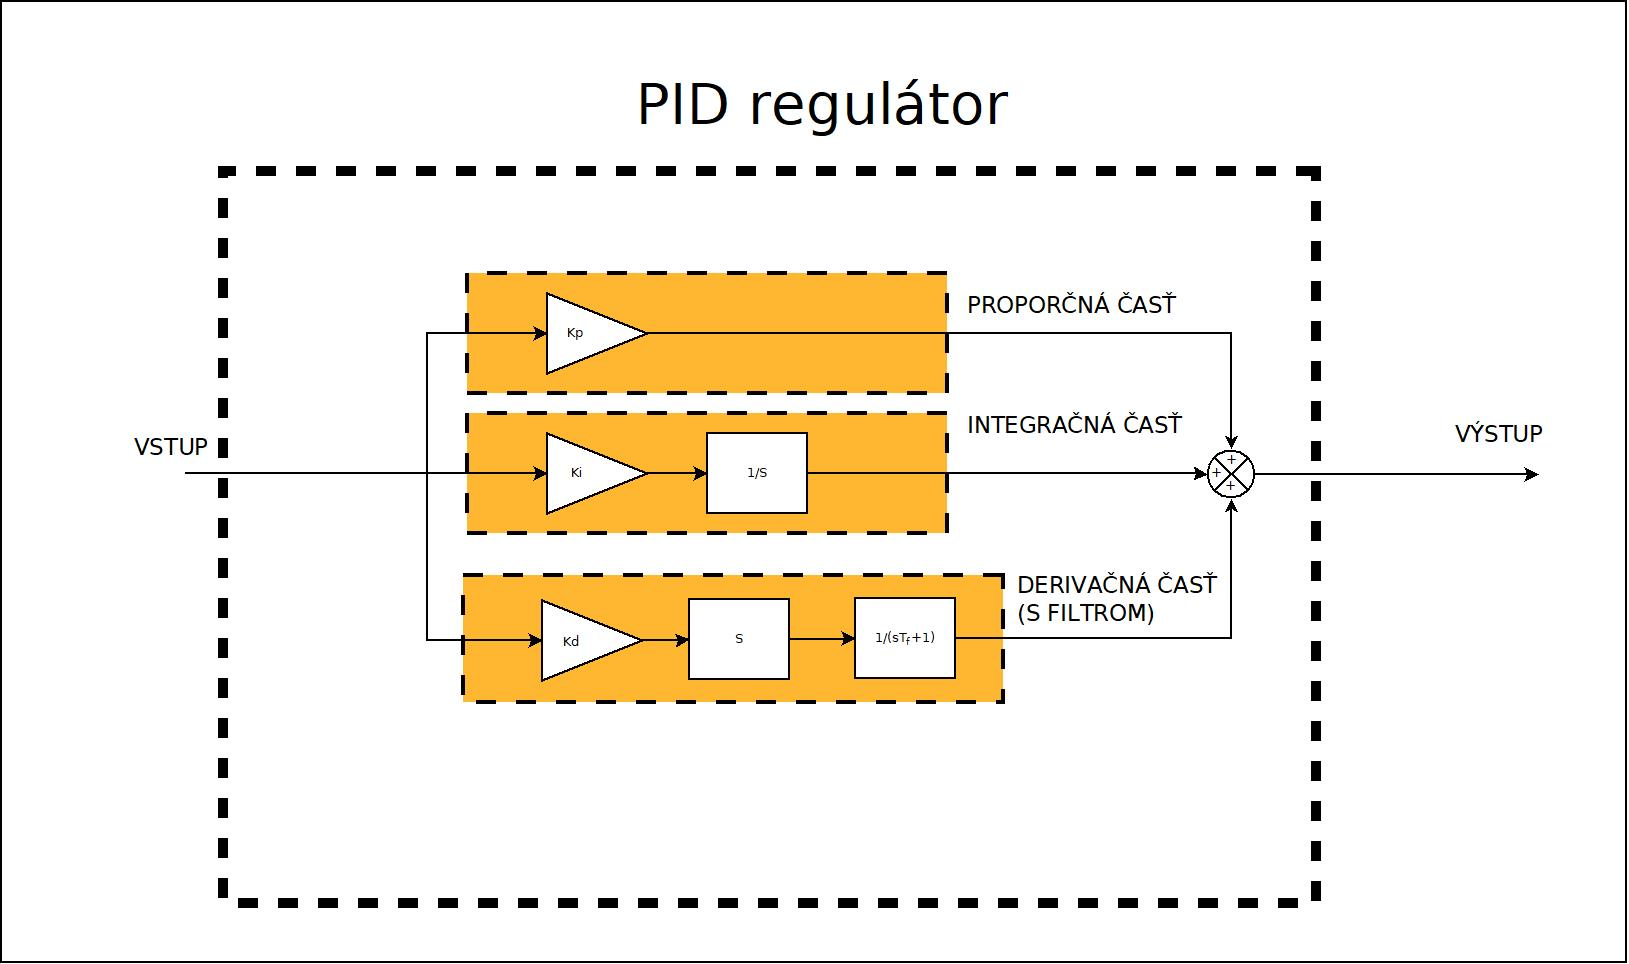
\includegraphics[width=8cm]{PIDComplete}
\caption{Štruktúra PID regulátora}
\label{fig:PIDComplete}
\end{figure}

Vychádzajúc z blokovej schémy na \figurename~\ref{fig:PIDComplete} môžeme podrobne opísať súčasti, z ktorých pozostáva PID.

\textbf {Proporčný člen} pozostáva zo zosilňovača, ktorý má na svojom výstupe Kp násobok chyby $e(t)$ . V praxi to teda znamená, že ak je reálny výstup regulovanej sústavy voči požiadavke značne veľký $\rightarrow$ chyba je veľká a záporná, teda proporčný člen reaguje veľkým záporným výstupom. Tento následne zníži veľkosť výstupu a teda aj odchýlku od požadovanej hodnoty. Matematicky je možné vyjadriť výstup proporčného člena ako:

\begin{equation}
u_p (t)= K_p e( t )
\end{equation}

kde up(t) predstavuje výstup a e(t) chybu na vstupe člena v čase t. 

Prípadne je ešte možné použiť vyjadrenie v Laplaceovej rovine vo forme prenosovej funkcie:

\begin{equation}
\dfrac {U_p(s)} {E(s)} = K_p 
\end{equation}
kde $UP(s)$ je výstup a $E(s)$ chyba, vyjadrené v Laplaceovej rovine.
\section{Kompilácia dokumentu}

\textbf{Integračný člen} reaguje na súčet chýb, naakumulovaných od spustenia regulátora. Tento súčet je následne vynásobený konštantou Ki a prenesený na výstup integračného bloku. Hlavnou výhodou integračnej časti je, že umožňuje PID reagovať aj na veľmi malé konštantné chyby, ktoré by proporčný člen inak nebol schopný korigovať. Aj tá najmenšia chyba voči požiadavke sa totiž procesom integrovania hromadí, až kým je výstup integračného člena dostatočný na jej skorigovanie. 

Matematické vyjadrenie integračného člena je:
\begin{equation}
u_i (t)= K_i \int_0^e \! e( t ) \, \mathrm{d}t 
\end{equation}
kde $u_i(t)$ predstavuje výstup integračného člena v čase $t$. 
Prenosová funkcia je:

\begin{equation}
\dfrac{U_i(s)}{E(s)}  = K_i\dfrac{ 1}{s} 
\end{equation}
kde $U_i (s)$ je výstup vyjadrený v Laplaceovej rovine.



Ďalšou možnosťou je použiť lokálnu inštaláciu LaTeX-u. Nevýhodou je, že inštalácie bývajú pomerne veľké a sťahujú sa po jednotlivých balíčkoch, čo zvykne trvať dosť dlho. Výhodou je, že lokálna inštalácia je lepšie konfigurovateľná a neaplikujú sa v nej podobné obmedzenia ako v prípade služby Overleaf -- napr. obmedzenie na počet súborov.

Jednou z populárnych distribúcií LaTeX-u je distribúcia TeX Live. Na Linux-e je ju typicky možné nájsť v balíčkovom systéme. Na Windows-e je možné zase použiť jednoduchý grafický inštalátor, ktorý možno stiahnuť na \href{https://www.tug.org/texlive/}{tug.org/texlive/}.

\section{Encxvlna a správne zalamovanie}

Slovenská typografia je charakteristická jednou mierne excentrickou požiadavkou -- že niektoré predložky a spojky nesmú byť na konci riadku. Ak sa tam vyskytnú, musia sa už zalomiť do nasledujúceho riadku. Na realizáciu tejto funkcionality v LaTeX-u je potrebné použiť balíček \texttt{encxvlna}. Drobná komplikácia spočíva v tom, že tento balíček vyžaduje aktiváciu systému \texttt{enctex}.

V inštalácii TeXLive je možné \texttt{enctex} aktivovať buď pre užívateľa alebo pre celý systém. V oboch prípadoch je na to potrebné vytvoriť súbor s názvom \texttt{fmtutil.cnf}, ktorý bude obsahovať:
\begin{Verbatim}
pdflatex pdftex language.dat -enc -translate-file=cp227.tcx *pdflatex.ini
\end{Verbatim}
Kľúčová je časť \texttt{-enc}, ktorá hovorí, že sa má povoliť \texttt{enctex}.

\subsection{Aktivácia \texttt{enctex}-u pre užívateľa}

V prípade aktivácie pre užívateľa je súbor \texttt{fmtutil.cnf} potrebné umiestniť do domovského adresára užívateľa, na cestu \texttt{texmf/web2c}.

Následne treba z príkazového riadku spustiť príkaz:
\begin{Verbatim}
fmtutil -user --all
\end{Verbatim}
ktorý nanovo prekompiluje užívateľské LaTeX formáty tak, že príkaz pdflatex bude mať aktivovaný \texttt{enctex}.

\subsection{Aktivácia \texttt{enctex}-u pre celý systém}

V prípade aktivácie pre celý systém sa súbor \texttt{fmtutil.cnf} umiestni do adresára LaTeX-ovej inštalácie, na cestu \texttt{texmf-local/web2c}. Následne je znovu potrebné prekompilovať LaTeX formáty, lenže systémové. Používa sa na to príkaz:
\begin{Verbatim}
fmtutil -sys --all
\end{Verbatim}
Keďže príkaz modifikuje systémovú inštaláciu, môže byť potrebné spustiť ho s administrátorskými privilégiami. Napr. na Ubuntu sa to dosiahne pomocou príkazu \texttt{sudo}.

\subsection{Overleaf a \texttt{enctex}}

V systéme Overleaf nie je enctex možné aktivovať -- preto na kompiláciu dokumentu je potrebné zakomentovať riadok \texttt{\textbackslash{usepackage}\{encxvlna\}} v \texttt{main.tex}.

\section{Includeonly}

V prípade rozsiahlejšieho dokumentu môže kompilácia do PDF trvať neprimerane dlho. Preto je užitočné niekedy dokument prestaviť tak, aby sa generovala len nejaká jeho menšia časť -- typicky jedna kapitola. To by však mohlo poškodiť odkazy na iné kapitoly, zmeniť číslovanie strán a pod. -- takže vygenerovaná kapitola by vyzerala inak než bude vyzerať vo finálnom texte.

Preto existuje prostredie \texttt{includeonly}, v rámci ktorého sa dá zadefinovať, z ktorých \texttt{.tex} súborov vložených pomocou makra \texttt{include} sa má aktuálne generovať. Pomocné súbory vygenerované z ostatných \texttt{.tex} súborov sú však stále k dispozícii a preto sa dajú čísla strán, odkazy a všetko ostatné v aktuálnom PDF realizovať korektne -- presne v takom tvare, ako to bude aj vo finálnej verzii.

Prostredie \texttt{includeonly} je už pripravené v súbore \texttt{main.tex} -- stačí ho odkomentovať a vložiť názvy tých súborov, z ktorých sa má aktuálne generovať PDF.
